\documentclass[12pt,a4paper,titlepage]{article}
\usepackage[utf8x]{inputenc}
\usepackage{amsfonts}
\usepackage{amsmath}
\usepackage{graphicx}
\usepackage{hyperref}
\hypersetup{
    colorlinks=false,
    pdfborder={0 0 0},
}
\usepackage{fancyvrb}
\usepackage{listings}
\usepackage{wrapfig}
\setlength{\headheight}{15pt}
\usepackage{titlesec}
\usepackage[left=35mm, right=25mm, top=25mm, bottom=25mm]{geometry}
\usepackage{fancyhdr}
\pagestyle{fancy}
\titleformat{\chapter}[display]
{\normalfont\huge\bfseries}{\ \ \thechapter}{20pt}{\Huge}

\usepackage[parfill]{parskip}
\author{Tom Blount}
\date{January 25, 2013}
\title{On the Implementation of Authentication Mechanisms for Mobile Devices over Wireless Networks}

\begin{document}
\maketitle

\tableofcontents
\newpage
\paragraph{Abstract}
This report gives an overview of the 802.1X specification and describes the design and implementation undertaking in this investigation. The report then covers an extension to this project, the 802.11r specification, used for fast switching between access points, and determines its overall feasibility.

\paragraph{Acknowledgements}
Thanks of course go to the other members of my group, José Cubero, Thomas Grainger and Chris Orchard.
Thanks also go to the Southampton University Wireless Society (SUWS) for lending us two wireless nodes.

\newpage
\section{Introduction}

\subsection{Brief}
The initial brief we were given was to: 
\textit{{\quote ``Design and demonstrate a simulation of the implementation of an efficient authentication protocol for mobile networks.''}}

After discussing amongst ourselves on the merits and drawbacks of various approaches to this task (including a number of extensions to the initial specification that we considered interesting avenues of research in their own right), we consulted J. Reeve and S.J. Braithwaite to confirm our approach was appropriate. From this discussion and the preceding brief, we extrapolated and defined the following requirements for the project, presented below in MoSCoW format.

\subsection{Requirements}
\begin{itemize}
\item[\textbf{Must}] Implement a simulated authentication protocol and demonstrate it working
\item[\textbf{Must}] Implement a working authentication protocol, using a single client, a single access point, and a single server and demonstrate it working
\item[\textbf{Should}] Demonstrate the use of an additional access point and the switching of the client between the two
\item[\textbf{Could}] Investigate the possibility of ``fast'' transitioning between access points
\end{itemize}

\newpage
\section{802.1X}
\subsection{Overview}
802.1X is a method of controlling access to a local area network at the data-link layer (layer two of the Open Systems Interconnection model) of the network. Three components are defined in the specification: the supplicant, the authenticator and the authentication server (see section \ref{sec:8021X;sub:components} for details).

Because 802.1X controls authentication through the data-link layer, local abuse within a wireless hotspot, for example, is prevented (as opposed to other authentication methods such as web-redirect). This also has the benefit of preventing unauthorised clients from being allocated an IP address -- this can be invaluable to campuses with few IPv4 addresses (even more so since the exhaustion of the IPv4 address space in January 2011 \cite{icaan11}).

\begin{figure}[h!]
\centering
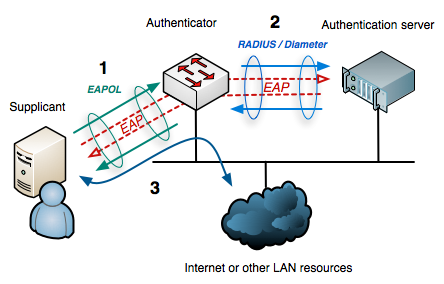
\includegraphics[scale=0.7]{./images/8021X.png}
\caption{An image of how 802.1X works over a (wired) network \cite{image8021X}}
\end{figure}

\subsection{Components}
\label{sec:8021X;sub:components}
\subsubsection{Authentication server}
The authentication server holds the credentials of clients, to determine if they should be granted access to the private section of the network (often the internet), or if their access has been revoked.

Despite there being alternative protocols for server/authenticator communication (such as Diameter\footnote{RFC 6733: http://www.ietf.org/rfc/rfc6733.txt} and TACACS\footnote{RFC 1492: http://www.ietf.org/rfc/rfc1492.txt}), RADIUS is the \textit{de facto} standard, used by many institutions (such as eduroam\footnote{http://www.eduroam.org/}) \cite{tipton04}.

The RADIUS protocol provides centralized AAA: Authentication, the ability to verify a user's identity via their credentials (e.g. a username and password); Authorisation, the ability to define different levels of access to users with different (predetermined) levels of clearance; and Accounting, the ability to track the access to and usage of these resources over periods of time and space.

\subsubsection{Authenticator}
The authenticator is usually a network switch or, in the case of wireless networks, an access point. Its role is to prevent unauthorised access to the private network ``behind'' it until a client is authenticated. To facilitate this, the authenticator relays messages from the client to the authentication server.

\subsubsection{Supplicant}
The supplicant can refer to both the client device wishing to be authenticated and to the software running on the client that actually provides it's authentication details to the authenticator.

\subsection{EAP}
802.1X also defines the use of Extensible Authentication Protocol (a framework for authentication communication via networks, defined in RFC 3748\footnote{http://www.ietf.org/rfc/rfc3748.txt}) over IEEE802 local area networks, or EAPOL. EAPOL is used to encapsulate EAP messages sent between the supplicant and authenticator.

EAP-Tunnelled Transport Layer Security (EAP-TTLS) is an EAP method that provides a degree of privacy and security for the client. The client first verifies the identity of the server using a PKI certificate (and, optionally, vice versa) and then establishes a secure tunnel between themselves and the authenticator using ``anonymous'' credentials. They can then send their actual credentials privately and securely through the tunnel.

\newpage
\section{Implementation}

\subsection{Overview}
The primary requirement of creating a simulated authentication could be completed by setting up a lone authentication server (see section \ref{sec:implementation;sub:components;sub:server} below) and running a virtual supplicant locally. This simulated messages passing from the supplicant via an authenticator and to the server.

The next stage was to implement the supplicant and authenticator in reality (see sections \ref{sec:implementation;sub:components;sub:accesspoint} and \ref{sec:implementation;sub:components;sub:client} below).

\subsection{Components}

\subsubsection{Server}
\label{sec:implementation;sub:components;sub:server}
Implementing (as well as debugging and testing) the authentication server made up the bulk of this author's individual contribution. The consisted of researching the appropriate server-side software, installing it on a virtual machine hosted by ECS and configuring it correctly. 

While there are many variants of RADIUS software, we chose \texttt{freeradius} due to its open-source nature and popularity, making it ideal for use in this project. The decision was made to install a RPM package that had been pre-built in a controlled environment.

Next, the configuration files must be updated with the appropriate system details. The essential items of configuration are determining the credentials of the users who will be accessing the system (their username, password and, crucially, whether they should be allowed or rejected), and the clients they will use (the IP address for example). In this case a user \texttt{TomB} was set to be authorised when using the password \texttt{TomBsPassword}. A second user, \texttt{TomG} was set to be always refused access (to demonstrate revoked credentials - see section \ref{sec:evaluation;sub:testing}). The next stage was to generate the necessary certificates that were used to identify the server (using EAP-TTLS). These were edited and made from within \texttt{raddb/certs/}. Finally, the appropriate EAP method needed to be configured, and pointed towards the generated certificates.

Example code from these key files can be found in appendix \ref{sec:Code;sub:radius}.

\subsubsection{Access point}
\label{sec:implementation;sub:components;sub:accesspoint}
We received on loan from the Southampton University Wireless Society (SUWS)\footnote{http://www.sown.org.uk} two ``Meraki Mini'' access points to use throughout the course of this project. The Meraki Mini has a 180MHz CPU and a 60mW 802.11b/g radio.
\begin{figure}[h!]
\centering
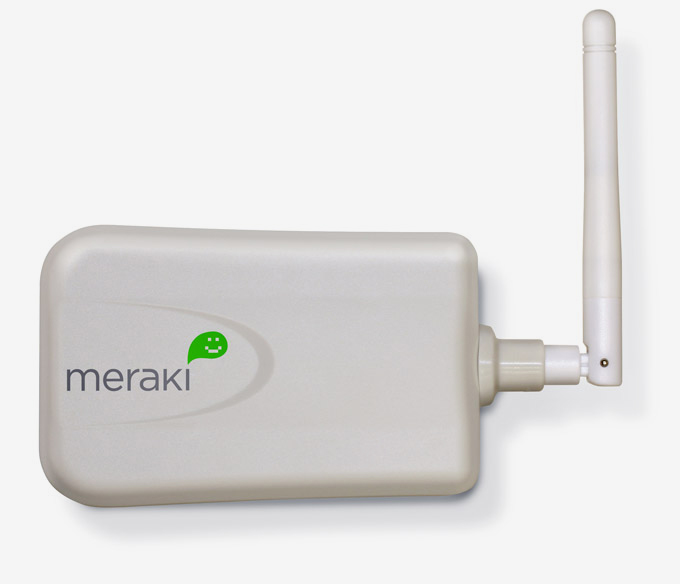
\includegraphics[scale=0.3]{./images/meraki-mini.jpg}
\caption{A Meraki Mini access point, similar to the ones used in this project \cite{imagemeraki}}
\end{figure}

However, instead of running the default Meraki firmware, the nodes were re-flashed to use \texttt{OpenWrt}\footnote{https://openwrt.org/}, a distribution of Linux, designed for use on embedded devices (these nodes were purchased before Meraki changed their EULA to prohibit such). This was used to build and run \texttt{hostapd} authenticator software\footnote{http://w1.fi/} which runs in user space, in the background, relaying messages from supplicant to server.

\subsubsection{Client}
\label{sec:implementation;sub:components;sub:client}
The client runs the supplicant software \texttt{wpa\_supplicant}. This must have the same credentials as those preprogrammed on the server and must be configured with the appropriate username and password combination. Some supplicant software includes a GUI allowing users to input these details at run time, but we chose to preconfigure ours - an example config file is provided in appendix \ref{sec:Code;sub:supplicant}.

\subsection{Challenges}
Throughout implementation we faced, and overcame, a number of challenges. Certainly one of the most arduous was attempting to configure the embedded devices with bleeding-edge software, as almost all programs needed to be cross-compiled. Another issue was that, as the authentication server was running as a virtual machine within ECS, the connection needed to be routed through a VPN (in this instance, one of our personal computers).

\newpage
\section{802.11r}

\subsection{Overview}
Developed in 2008, the 802.11r specification amends the 802.11 ``WiFi'' specification to allow fast Basic Service Set transitions (FTs) -- in other words, it is designed to allow a mobile device to be quickly and securely transferred between access points. To achieve this, instead of renegotiating a new session and key after every transfer, part of the key is cached to allow further communication after transferring access points for some amount of time.

While this is, of course, desirable for any mobile network it is particularly important given the recent proliferation of internet-capable smart phones and Voice Over IP (VOIP) technology.

\subsection{Implementation}
Implementing this protocol involved recompiling both the authenticator (\texttt{hostapd}) and supplicant (\texttt{wpa\_supplicant}) to support 802.11r, and configuring them accordingly. The utility \texttt{wpa\_cli} could then be used to interact with \texttt{wpa\_supplicant} and force the supplicant to roam to a new access point.

Unfortunately however, during testing we could not get the fast transition to occur. As can be seen in appendix \ref{sec:testing-output;sub:80211r}, the line \texttt{FT: Invalid group cipher (0)} which translates as the program receiving \texttt{WPA\_CIPHER\_NONE}. This state should not be reachable with the given configuration (it should be either \texttt{WPA\_CIPHER\_CCMP} or \texttt{WPA\_CIPHER\_TKIP} at this stage) and was possibly caused by bugs introduced by the bleeding-edge software used - regrettably there was not enough time remaining at this stage of the project to determine and fix the root cause.

\newpage
\section{Evaluation}

\subsection{Testing}
\label{sec:evaluation;sub:testing}
Each of the implemented sections were tested incrementally, using a command line tool bundled with \texttt{wpa\_supplicant} called \texttt{eapol\_test}. This allows simulated EAP messages to be sent to a server, based on settings in a configuration file (specifying the EAP method, username, password, etc.) and the responses to be examined in detail. 

The output from testing the server (and the simulated authenticator and supplicant) can be seen in appendix \ref{sec:testing-output;sub:simulation} - the server is shown on the left (in debug mode, to produce the most detailed output) and the \texttt{eapol\_test} on the right. Initially a valid user attempted to connect and was successfully authenticated. Next, a valid user with revoked attempted to connect and was refused access. Other tests of this nature (such as a valid user, with incorrect credentials) were performed and passed.

Once the authenticator and supplicant were implemented fully, these were also tested (and debugged as necessary) with \texttt{eapol\_test}. They were then run in a live environment repeating the above tests - a sample of the output is shown in appendix \ref{sec:testing-output;sub:supplicant}.

\subsection{Conclusions}
Overall, the project was a resounding success. We managed to implement not only a simulated authentication service, but a live demonstration of an efficient system with multiple hardware components. Although the proposed 802.11r extension was not fully implemented, the research into the protocol raised some interesting ideas for future work.

\subsection{Recommendations for future work}
The clear next stage for further development would be to fully implement an instance of 802.11r, and demonstrate the possible fast switching between access points. Ideally, a comparison could be drawn between the time taken using fast BSS and the transfers shown in this project, potentially with a practical demonstration of running a VOIP call during the transfer.

\newpage
\begin{thebibliography}{99}

\bibitem{icaan11} ICAAN, \textit{Available Pool of Unallocated IPv4 Internet Addresses Now Completely Emptied}, ICAAN News Release, February 2011

\bibitem{image8021X} Image by Arran Cudbard-Bell

\bibitem{tipton04}
H.F. Tipton and M. Krause, ``Centralized Authentication Services'', in \textit{Information Security Management Handbook}, 5xth ed. CRC Press, 2004, pp. 99.

\bibitem{imagemeraki}
M. Honan, \textit{Meraki Mini Serves Up Hot Heaping Wi-Fi}, Wired, September 2007. Available: http://www.wired.com/images/productreviews/2008/09/meraki\_mini\_f.jpg

\end{thebibliography}

\newpage
\appendix
\section{Example Code}

\subsection{RADIUS Server}
\label{sec:Code;sub:radius}

\subsubsection{raddb/users}
\begin{Verbatim}[frame=single]
#Give access to this user
TomB    Cleartext-Password := "TomBsPassword"
        Reply-Message = "Hello there %{User-Name}! How's it going?"

#Don't give access to this user
TomG    Auth-Type := Reject
        Reply-Message = "Oh no you don't Grainger. Not again."
\end{Verbatim}

\subsubsection{raddb/clients.conf}
\begin{Verbatim}[frame=single]
client linuxproj {
    ipaddr = 152.78.71.57
    secret = testing123
    require_message_authenticator = no
    
    #Used to specify a specific Network Access Server type
    #(e.g. cisco, multitech, etc.)
    nastype = other
}
\end{Verbatim}

\subsubsection{raddb/eap.conf}
\begin{Verbatim}[frame=single]
tls {
    certdir = ${confdir}/certs
    cadir = ${confdir}/certs
    private_key_password = whatever
    private_key_file = ${certdir}/server.pem
    certificate_file = ${certdir}/server.pem
    CA_file = ${cadir}/ca.pem
    dh_file = ${certdir}/dh
    random_file = ${certdir}/random
    CA_path = ${cadir}
    cipher_list = "DEFAULT"
}

ttls {
    default_eap_type = md5
    copy_request_to_tunnel = no
    use_tunneled_reply = no
    virtual_server = "inner-tunnel"
}
\end{Verbatim}

\subsection{Authenticator}
\label{sec:Code;sub:authenticator}

\subsubsection{hostapd.conf}
\begin{figure}[h!]
\begin{Verbatim}[frame=single]
auth_server_addr=152.78.61.5
auth_server_port=1812
auth_server_shared_secret=testing123
disable_pmksa_caching=1
okc=0
nas_identifier=kanga-cso1g09e
eapol_key_index_workaround=1
ieee8021x=1
wpa_key_mgmt=FT-EAP WPA-EAP
auth_algs=1
wpa=2
wpa_pairwise=CCMP
ssid=notthebees
bridge=br-lan
wmm_enabled=1
bssid=00:18:0a:01:3f:38
ignore_broadcast_ssid=0
mobility_domain=a1b2
r0_key_lifetime=100000
r1_key_holder=000102030406
reassociation_deadline=1000
r0kh=00:18:0a:01:3f:3f kanga-cso1g09e
	000102030405060708090a0b0c0d0e0f
r1kh=00:18:0a:01:3f:3f 00:01:02:03:04:05
	000102030405060708090a0b0c0d0e0f
r1kh=00:18:0a:01:3f:38 00:01:02:03:04:06
	000102030405060708090a0b0c0d0e0e
\end{Verbatim}
\caption{Code snippet by Chris Orchard}
\end{figure}

\subsection{Supplicant}
\label{sec:Code;sub:supplicant}

\subsubsection{wpa\_supplicant.conf}
\begin{figure}[h!]
\begin{Verbatim}[frame=single]
ctrl_interface=/var/run/wpa_supplicant
eapol_version=1
ap_scan=1
fast_reauth=1

network={
        ssid="notthebees"
        scan_ssid=1
        key_mgmt=FT-EAP WPA-EAP
        pairwise=CCMP
        group=CCMP
        eap=TTLS
        identity="TomB"
        anonymous_identity="anon"
        password="TomBsPassword"
        phase2="auth=PAP"
}
\end{Verbatim}
\caption{Code snippet by Thomas Grainger}
\end{figure}

\newpage
\section{Testing Output}

\subsection{Simulation}
\label{sec:testing-output;sub:simulation}
\begin{figure}[h!]
\centering
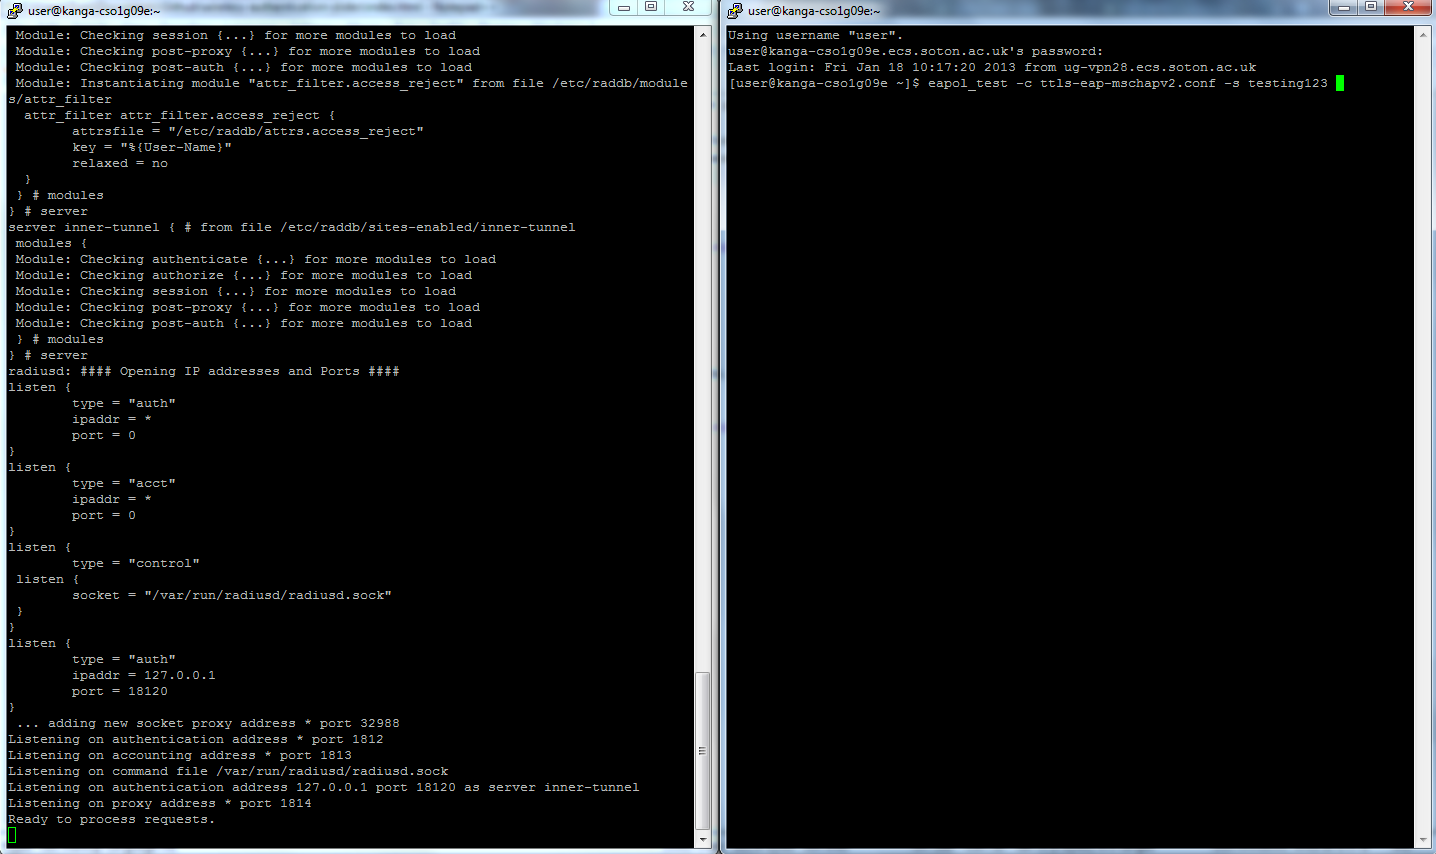
\includegraphics[scale=0.3]{./images/simulation/test1.png}
\caption{Setting up the server for testing}
\end{figure}

\begin{figure}[h!]
\centering
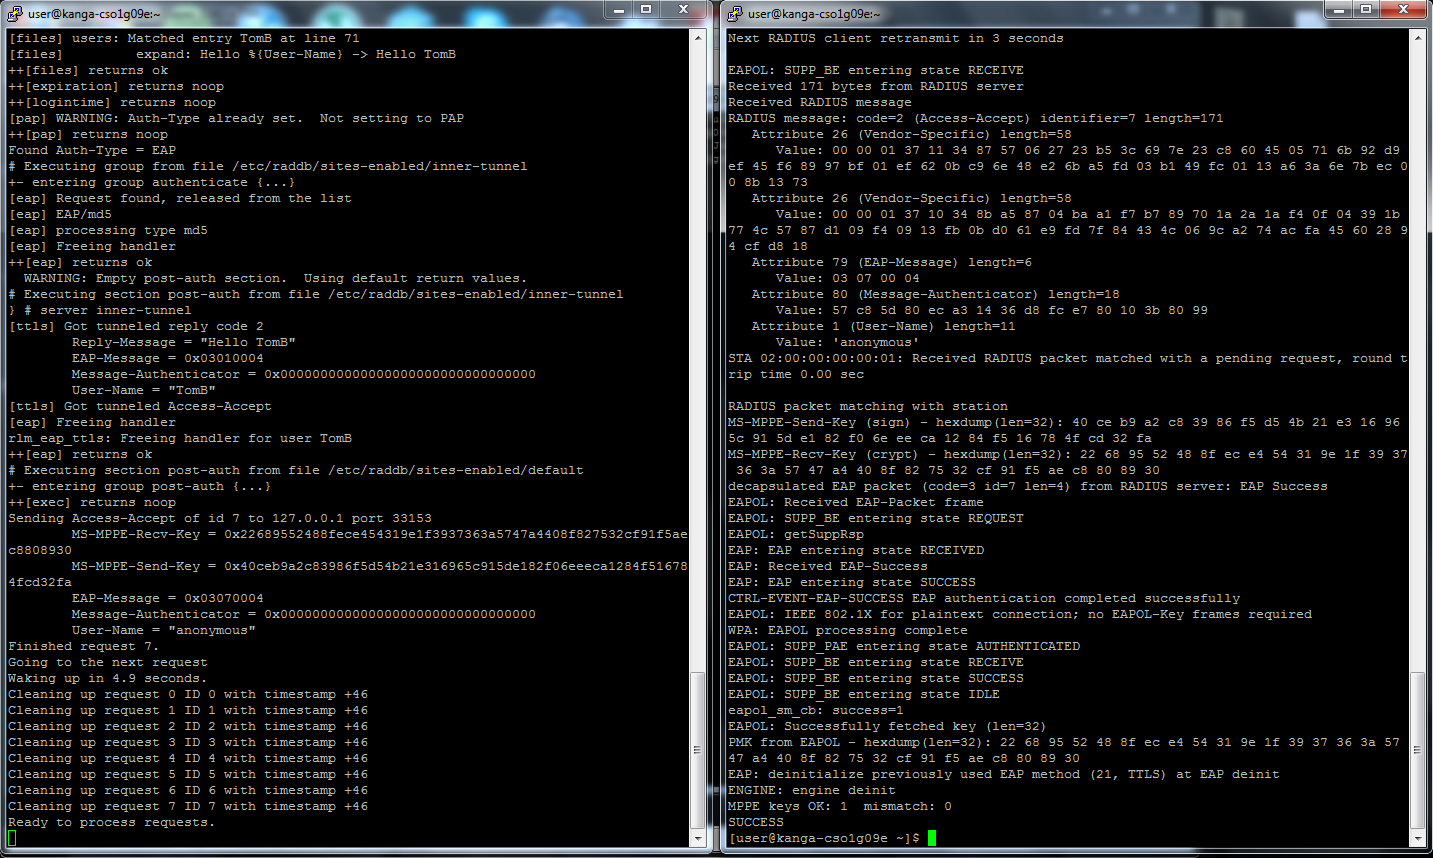
\includegraphics[scale=0.3]{./images/simulation/test2.png}
\caption{Connecting with valid credentials}
\end{figure}

\begin{figure}[h!]
\centering
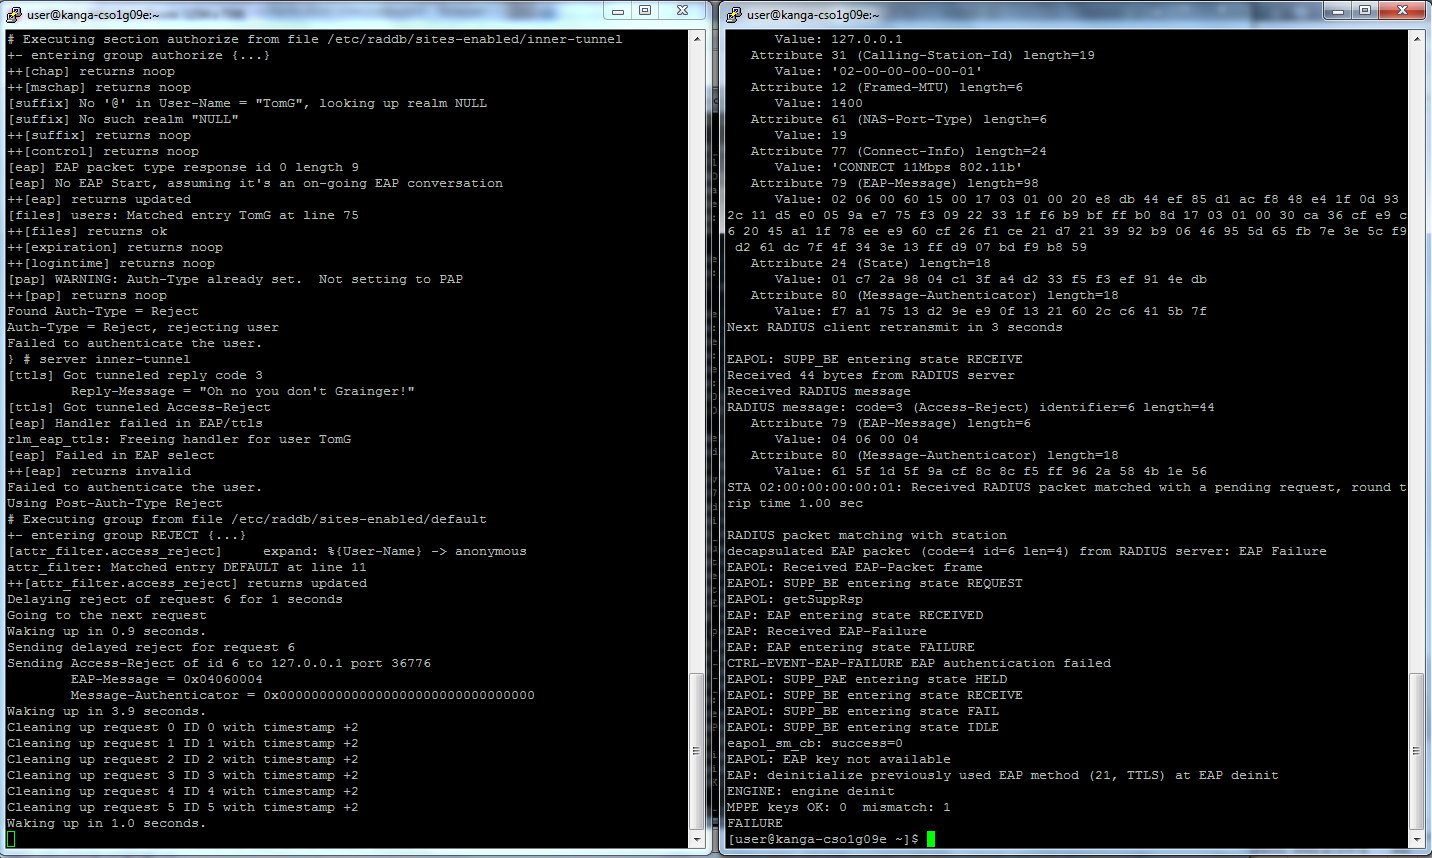
\includegraphics[scale=0.3]{./images/simulation/test3.png}
\caption{Connecting with invalid credentials}
\end{figure}

\subsection{wpa\_supplicant output}
\label{sec:testing-output;sub:supplicant}
\begin{figure}[h!]
\begin{Verbatim}[frame=single]
<3>SME: Trying to authenticate with 00:18:0a:01:3f:38
	(SSID='notthebees' freq=2412 MHz)
<3>Trying to associate with 00:18:0a:01:3f:38
	(SSID='notthebees' freq=2412 MHz)
<3>SME: Trying to authenticate with 00:18:0a:01:3f:3f
	(SSID='notthebees' freq=2462 MHz)
<3>Trying to associate with 00:18:0a:01:3f:3f
	(SSID='notthebees' freq=2462 MHz)
<3>Associated with 00:18:0a:01:3f:3f
<3>CTRL-EVENT-EAP-STARTED EAP authentication started
...
<3>CTRL-EVENT-EAP-SUCCESS EAP authentication completed successfully
<3>WPA: Key negotiation completed with 00:18:0a:01:3f:3f
	[PTK=CCMP GTK=CCMP]
<3>CTRL-EVENT-CONNECTED - Connection to 00:18:0a:01:3f:3f
	completed (reauth) [id=0 id_str=]
> roam 00:18:0a:01:3f:38
OK
<3>SME: Trying to authenticate with 00:18:0a:01:3f:38
	(SSID='notthebees' freq=2412 MHz)
<3>Trying to associate with 00:18:0a:01:3f:38
	(SSID='notthebees' freq=2412 MHz)
<3>Associated with 00:18:0a:01:3f:38
<3>CTRL-EVENT-EAP-STARTED EAP authentication started
...
<3>CTRL-EVENT-EAP-SUCCESS EAP authentication
	completed successfully
<3>WPA: Key negotiation completed with 00:18:0a:01:3f:38
	[PTK=CCMP GTK=CCMP]
<3>CTRL-EVENT-CONNECTED - Connection to 00:18:0a:01:3f:38
	completed (reauth) [id=0 id_str=]
\end{Verbatim}
\caption{Code snippet by Thomas Grainger}
\end{figure}

\subsection{802.11r output}
\label{sec:testing-output;sub:80211r}
\begin{figure}[h!]
\begin{Verbatim}[frame=single]
wlan0: Trying to associate with 00:18:0a:01:3f:38
	(SSID='notthebees' freq=2412 MHz)
FT: Invalid group cipher (0)
wlan0: Authentication with 00:18:0a:01:3f:38 timed out.
wlan0: Trying to associate with 00:18:0a:01:3f:3f
	(SSID='notthebees' freq=2462 MHz)
wlan0: Authentication with 00:18:0a:01:3f:3f timed out.
wlan0: Trying to associate with 00:18:0a:01:3f:3f
	(SSID='notthebees' freq=2462 MHz)
wlan0: Authentication with 00:18:0a:01:3f:3f timed out.
wlan0: Trying to associate with 00:18:0a:01:3f:38
	(SSID='notthebees' freq=2412 MHz)
^Cwlan0: CTRL-EVENT-TERMINATING - signal 2 received
\end{Verbatim}
\caption{Code snippet by Thomas Grainger}
\end{figure}

\end{document}